\documentclass[11pt]{beamer}

\usepackage{cedilleverbatim}
\usepackage{stmaryrd}
\usepackage{MnSymbol}
\usepackage[normalem]{ulem}
%\usepackage[utf8]{inputenc}

\usepackage{tikz}
\usepackage{mathtools}
\usepackage{color}
\usepackage{pgflibraryarrows}
\usepackage{pgflibraryshapes}
\usetikzlibrary{decorations.text}

\usepackage{latexsym}

\mode<presentation>{\usetheme{Boston}}
\usepackage[english]{babel}
\usepackage{times}
\usepackage[T1]{fontenc}

%\definecolor{colorced}{RGB}{255,128,0}
\definecolor{colorced}{RGB}{255,0,0}
%\definecolor{colorcedc}{RGB}{0,128,255}
%\definecolor{colorcedc}{RGB}{96,96,96}
\definecolor{colorcedcore}{RGB}{0,128,255}
\definecolor{colorcedmode}{RGB}{128,0,255}

\newcommand{\cedtext}[1]{\emph{$\texttt{#1}$}}
\newcommand{\lamxxx}[0]{$\lambda$ x$.$ x x}

\newcommand{\cedillearchitectureframe}[1]{
\hspace{1cm}
\begin{tikzpicture}

\path (1,2.5) node[very thick,colorcedmode,ellipse,draw,inner xsep=5pt,inner ysep=20pt](emacsmode){Emacs mode} ;
\path (6,2.5) node[very thick,colorced,ellipse,draw,inner xsep=5pt,inner ysep=20pt](backend){Backend} ;

\path (-1.3,4) node[thick,orange,ellipse,draw,inner xsep=3pt,inner ysep=6pt](cedfilesa){{\small .ced files}} ;

\draw[<->,very thick,black] (emacsmode.east) -- (backend.west);
\draw[->,thick,black] (cedfilesa.south east) -- (emacsmode.north west);

#1

\path (6,0) node[thick,orange,ellipse,draw,inner xsep=3pt,inner ysep=6pt](cedfilesb){{\small .ced files}} ;

\path (2.5,0) node[very thick,colorcedcore,ellipse,draw,inner xsep=3pt,inner ysep=6pt](cedillecore){{\small Cedille\textsubscript{core}}} ;
\path (0.9,0.7) node[thick,colorcedcore,ellipse,inner xsep=2pt,inner ysep=2pt](cedillecoreok){{\small Ok}} ;
\path (0.75,-0.7) node[thick,colorcedcore,ellipse,inner xsep=2pt,inner ysep=2pt](cedillecoreerr){{\small Error}} ;

\draw[->,thick,black,dashed] (backend.south) -- (cedfilesb.north);
\draw[->,thick,black] (cedfilesb.west) -- (cedillecore.east);
\draw[->,thick,black] (cedillecore.north west) -- (cedillecoreok.south east);
\draw[->,thick,black] (cedillecore.south west) -- (cedillecoreerr.north east);

\end{tikzpicture}
}

\newcommand{\checkagainst}[2]{
\textcolor{black}{\cedtext{#2}}

%\vspace{-0.1cm}

\textcolor{black}{$\Downarrow$}

%\vspace{0.1cm}

\textcolor{colorced}{\cedtext{#1}}
%\textcolor{black}{\hspace{0.1cm} $\Leftarrow$ \hspace{0.1cm} #2}
}

\newcommand{\elabrule}[4]{
\begin{frame}[t]
\frametitle{\textcolor{colorced}{Cedille} $\leadsto$ \textcolor{colorcedcore}{Cedille Core}$:$ {#1}}
\vspace{1cm}
\textcolor{darkgray}{\cedtext{$\Gamma$ $=$ \cedtext{#2}}}
\noindent\rule{\textwidth}{0.2pt}

\vfill
\begin{center}
#3

$\leadsto$

\textcolor{colorcedcore}{\cedtext{#4}}

\end{center}
\vfill

\end{frame}
}

\newcommand{\elabruleb}[6]{
\begin{frame}[t]
\frametitle{\textcolor{colorced}{Cedille} $\leadsto$ \textcolor{colorcedcore}{Cedille Core}$:$ {#1}}
\vspace{1cm}
\textcolor{darkgray}{\cedtext{$\Gamma$ $=$} \cedtext{#2}}
\newline
\qquad\textcolor{darkgray}{\qquad\cedtext{#3}}
\noindent\rule{\textwidth}{0.2pt}

\vfill
\begin{center}
#4

$\leadsto$

\textcolor{colorcedcore}{\cedtext{#5}}

\textcolor{colorcedcore}{\cedtext{#6}}

\end{center}
\vfill

\end{frame}

}



\date{\ }


\begin{document}

\setbeamercolor{normal text}{bg=white,fg=black}

\begin{frame}

\begin{center}

{\Huge \texttt{cedille}}

\vspace{1cm}

{\Large \textcolor{red}{Tooling: Interactive Commands}}

\end{center}

\end{frame}




\begin{frame}
\frametitle{Interactive Commands}
\begin{itemize}
\item Backend sends all data in one batch
\pause
\item Sometimes we want more information than was given, but wouldn't be realistic to include for all nodes
\pause
\item Hence the need for ``Interactive'' Commands
\pause
\item Node Commands
\pause
\begin{itemize}
\item ``C-i n'' -- Normalize
\pause
\item ``C-i h'' -- Head-normalize
\pause
\item ``C-i e'' -- Erase
\end{itemize}
\pause
\item Beta-Reduction Commands
\pause
\begin{itemize}
\item ``C-i b'' -- Prompt for expression to open in beta-reduction buffer
\pause
\item ``C-i t'' -- Use selected node's type in beta-reduction buffer
\pause
\end{itemize}

\end{itemize}

\end{frame}



\begin{frame}
\frametitle{Interactive Commands: Beta-Reduction Buffer}
\begin{itemize}
\item Navigation commands (``f'', ``b'', ``n'', ``p'', etc...)
\pause
\item ``C-i n'' -- Normalize and replace the selected node
\item ``C-i h'' -- Head-normalize and replace the selected node
\pause
\item ``C-i r'' -- Prompt for proof of equation, and rewrite the selected node with it
\pause
\item ``C-i p'' -- Reconstruct proof from steps taken
\pause
\end{itemize}

\end{frame}



\begin{frame}

\frametitle{Interactive Commands: One More}
\begin{itemize}
\item ``E'' -- Elaborate to Cedille Core
\end{itemize}
\end{frame}

\begin{frame}

\begin{center}

{\Huge $\leadsto$ \texttt{cedille}$_{\texttt{core}}$}

\vspace{1cm}

{\Large \textcolor{red}{Elaboration to Cedille Core}}

\end{center}

\end{frame}



\begin{frame}
\frametitle{What is Cedille Core?}

\begin{itemize}
\item Independent implementation of CDLE
\item Full annotations required
  \begin{itemize}
    \item No type inference
    \item No bidirectionality
  \end{itemize}
\item More verbose, much easier to check
\item Fewer than 1000 lines of Haskell code
\end{itemize}

\end{frame}

\begin{frame}
\frametitle{Architecture of Cedille}
\cedillearchitectureframe{\pause}
\end{frame}


\begin{frame}
\frametitle{\textcolor{colorced}{Cedille} vs. \textcolor{colorcedcore}{Cedille Core}}

\hspace{0.5cm}
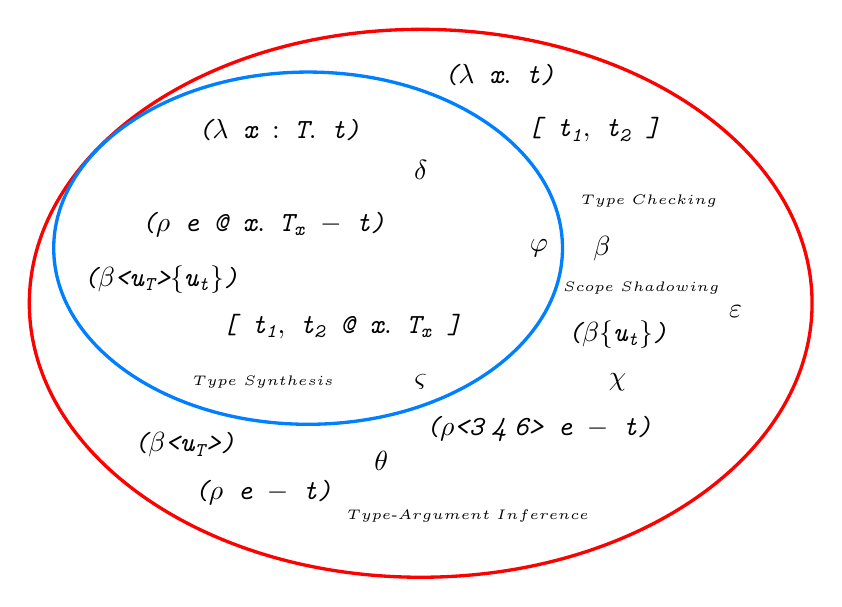
\begin{tikzpicture}

\path (0,0) node[very thick,colorced,ellipse,draw,inner xsep=100pt,inner ysep=70pt](cedille){} ;

\path (-1.8,2.2) node {\cedtext{($\lambda$ x $:$ T$.$ t)}} ;
\path (1,2.9) node {\cedtext{($\lambda$ x$.$ t)}} ;
\path (2.2,2.2) node {\cedtext{[ t\textsubscript{1}$,$ t\textsubscript{2} ]}} ;
\path (-1,-0.3) node {\cedtext{[ t\textsubscript{1}$,$ t\textsubscript{2} @ x$.$ T\textsubscript{x} ]}} ;
\path (4,-0.1) node {\cedtext{$\varepsilon$}} ;
\path (0,1.7) node {\cedtext{$\delta$}} ;
\path (-2,1) node {\cedtext{($\rho$ e @ x$.$ T\textsubscript{x} $-$ t)}} ;
\path (2.3,0.7) node {\cedtext{$\beta$}} ;
\path (-3,-1.8) node {\cedtext{($\beta$<u\textsubscript{T}>)}} ;
\path (2.5,-0.4) node {\cedtext{($\beta$\{u\textsubscript{t}\})}} ;
\path (-3.3,0.3) node {\cedtext{($\beta$<u\textsubscript{T}>\{u\textsubscript{t}\})}} ;
\path (1.5,0.7) node {\cedtext{$\varphi$}} ;
\path (-2,-2.4) node {\cedtext{($\rho$ e $-$ t)}} ;
\path (1.5,-1.6) node {\cedtext{($\rho$<3\;4\;6> e $-$ t)}};
\path (2.5,-1) node {\cedtext{$\chi$}} ;
\path (0,-1) node {\cedtext{$\varsigma$}} ;
\path (-0.5,-2) node {\cedtext{$\theta$}} ;
\path (0.6,-2.7) node {\tiny{$Type$-$Argument \ Inference$}} ;
\path (2.9,1.3) node {\tiny{$Type \ Checking$}} ;
\path (-2,-1) node {\tiny{$Type \ Synthesis$}} ;
\path (2.8,0.2) node {\tiny{$Scope \ Shadowing$}} ;

\pause

\path (-1.43,0.7) node[very thick,colorcedcore,ellipse,draw,inner xsep=65pt,inner ysep=45pt](cedillecore){} ;


% \pause messes up page number in bottom right corner--instead I am using \onslide<1-> as suggested by Joachim Breitner at https://tex.stackexchange.com/questions/21512/pause-in-tikzpicture-breaks-footline/70051
\onslide<1->

\end{tikzpicture}


\end{frame}



%\begin{frame}
%\frametitle{\textcolor{colorced}{Cedille} $\leadsto$ \textcolor{colorcedcore}{Cedille Core}}
%
%\begin{itemize}
%\item Classify $\lambda$-terms \\
%\quad \cedtext{\textcolor{colorced}{$\lambda$ x$.$ t}  $\leadsto$  \textcolor{colorcedcore}{$\lambda$ x $:$ T$.$ t}}
%\pause
%\item Insert inferred type arguments \\
%\quad \cedtext{\textcolor{colorced}{id zero}  $\leadsto$  \textcolor{colorcedcore}{id · Nat zero}}
%\pause
%\item Provide dependent type of second projection in $\iota$\hspace{0.02cm}-pairs \\
%\quad \cedtext{\textcolor{colorced}{[\! zero'$,$ zeroi\! ]} $\leadsto$ \textcolor{colorcedcore}{[\! zero'$,$ zeroi @ x$.$ NatI x\! ]}}
%\pause
%\item Ensure $\beta$-terms supply both a term \cedtext{u} for proving \cedtext{\{ u $\simeq$ u \}} and one for erasure \\
%\quad \cedtext{\textcolor{colorced}{$\beta$}  $\leadsto$  \textcolor{colorcedcore}{$\beta$<u>\{$\lambda$ x$.$ x\}}}
%\pause
%\item Convert δ-contradictions to Church-encoded \cedtext{\{ tt $\simeq$ ff \}} \\
%{\footnotesize \cedtext{\textcolor{colorced}{\{suc n $\simeq$ zero\}} $\leadsto$ \textcolor{colorcedcore}{\{suc n ff ($\lambda$ \_$.$ tt) $\simeq$ zero ff ($\lambda$ \_$.$ tt)\}}}}
%\pause
%\item Specify where rewrites occur in $\rho$-terms \\
%\quad \cedtext{\textcolor{colorced}{$\rho$ e $-$ t}  $\leadsto$  \textcolor{colorcedcore}{$\rho$ e @ x$.$ T\textsubscript{x} $-$ t}}
%\pause
%\begin{itemize}
%\item Rewriting is \uline{not} guaranteed to preserve typeability!
%\pause
%\end{itemize}
%\end{itemize}
%\end{frame}

\elabrule
  {$\lambda$-terms}
  {X $: \ \star$}
  {\checkagainst{$\lambda$ x$.$ x}{X $\rightarrow$ X}}
  {$\lambda$ x $:$ X. x}

\elabrule
  {$\iota$\hspace{0.02cm}-pairs}
  {A $:$ $\star$, B $:$ (A $\rightarrow$ $\star$), a $:$ A, b $:$ B a}
  {\checkagainst{[ a, b ]}{$\iota$ x $:$ A. B x}}
  {[ a, b @ x$.$ B x ]}

\elabrule
  {$\beta$-terms}
  {T $:$ $\star$, t $:$ T}
  {\checkagainst{$\beta$}{\{ t $\simeq$ t \}}}
  {$\beta$<t>\{$\lambda$ x$.$ x\}}

\elabrule
  {$\delta$-contradictions}
  {n $:$ Nat}
  {\textcolor{colorced}{\cedtext{\{ suc n $\simeq$ zero \}}}}
  {\{ suc n ff ($\lambda$ \_$.$ tt) $\simeq$ zero ff ($\lambda$ \_$.$ tt) \}}

\elabrule
  {$\rho$-terms}
  {m $:$ Nat, n $:$ Nat, e $:$ \{ suc m $\simeq$ n \}}
  {\checkagainst{$\rho$ e $-$ $\beta$}{\{ suc (suc m) $\simeq$ suc n \}}}
  {$\rho$ e @ x$.$ \{ suc x $\simeq$ suc n \} $-$ $\beta$<suc n>\{$\lambda$ x$.$ x\}}

%\elabrule
%  {$\rho$-terms \textcolor{white}{Invisible A}}
%  {A $:$ $\star$, B $:$ A $\rightarrow$ $\star$, a $:$ A, e $:$ \{ a $\simeq$ \lamxxx \}}
%  {\checkagainst{$\rho$ e $-$ $\lambda$ b$.$ b}{B a $\rightarrow$ B a}}
%  {$\rho$ e @ x$.$ (B x $\rightarrow$ B x) $-$ $\lambda$ b $:$ B (\textcolor{white}{$\underbrace{\text{\cedtext{\textcolor{colorcedcore}{\lamxxx}}}}_{}$})$.$ b}

\elabrule
  {$\rho$-terms \textcolor{white}{Invisible B}}
  {A $:$ $\star$, B $:$ (A $\rightarrow$ $\star$), a $:$ A, e $:$ \{ a $\simeq$ \lamxxx \}}
  {\checkagainst{$\rho$ e $-$ $\lambda$ b$.$ b}{B a $\rightarrow$ B a}}
  {$\rho$ e @ x$.$ (B x $\rightarrow$ B x) $-$ $\lambda$ b $:$ B (\hspace{-18pt}$\underbrace{\text{\lamxxx}}_{\text{$\phi$ e $-$ a \{\lamxxx\}}}$\hspace{-18pt})$.$ b}

%\elabrule
%  {$\rho$-terms \textcolor{white}{Invisible C}}
%  {A $:$ $\star$, B $:$ A $\rightarrow$ $\star$, a $:$ A, e $:$ \{ a $\simeq$ \lamxxx \}}
%  {\checkagainst{$\rho$ e $-$ $\lambda$ b$.$ b}{B a $\rightarrow$ B a}}
%  {\hspace{-0.4cm}$\rho$ e @ x$.$ (B x $\rightarrow$ B x) $-$ $\lambda$ b $:$ B ($\underbrace{\text{$\phi$ e $-$ a \{\lamxxx\}}}_{\text{$\Leftarrow$ A}}$)$.$ b}

\elabruleb
  {$\rho$-terms \textcolor{white}{Invisible D}}
  {A $:$ $\star$, B $:$ ($\Pi$ a $:$ A$.$ $\Pi$ a' $:$ A$.$ \{ a $\simeq$ a' \} $\rightarrow$ $\star$),}
  {a $:$ A, a'\! $:$ A, e $:$ \{\!\! a\! $\simeq$\! a'\!\! \}, p $:$ \{\! a\! $\simeq$\! \lamxxx\! \}}
  {\checkagainst{$\rho$ p $-$ $\lambda$ b$.$ b}{B a a' e $\rightarrow$ B a a' e}}
  {$\rho$ e @ x$.$ (B x a' e $\rightarrow$ B x a' e) $-$}
  {$\lambda$ b $:$ B ($\phi$ p $-$ a \{\lamxxx\}) a'\!\! \hspace{-50pt}$\underbrace{\text{e}}_{\text{$\rho$ $\varsigma$ p @ x$.$ \{\! x $\simeq$ a'\!\! \} $-$ e}}$\hspace{-50pt}$.$ b}

%\elabruleb
%  {$\rho$-terms \textcolor{white}{Invisible E}}
%  {A $:$ $\star$, B $:$ $\Pi$ a $:$ A$.$ $\Pi$ a' $:$ A$.$ \{ a $\simeq$ a' \} $\rightarrow$ $\star$,}
%  {a $:$ A, a'\! $:$ A, e $:$ \{\!\! a\! $\simeq$\! a'\!\! \}, p $:$ \{\! a\! $\simeq$\! \lamxxx\! \}}
%  {\checkagainst{$\rho$ p $-$ $\lambda$ b$.$ b}{B a a' e $\rightarrow$ B a a' e}}
%  {$\rho$ e @ x$.$ (B x a' e $\rightarrow$ B x a' e) $-$}
%  {\hspace{-0.8cm}$\lambda$ b $:$ B ($\phi$ p $-$ a \{\lamxxx\}) a' ($\underbrace{\text{$\rho$ $\varsigma$ p @ x$.$ \{\! x $\simeq$ a'\!\! \} $-$ e}}_{\Leftarrow \ \text{\{ \lamxxx $\ \simeq$ a' \}}}$)$.$ b}

\elabrule
  {Type Inference}
  {id $:$ ($\forall$ X $:$ $\star.$ X $\rightarrow$ X)}
  {\textcolor{colorced}{\cedtext{id zero}}}
  {id · Nat zero}
  


%\begin{frame}
%\frametitle{Type-Preserving Rewrites: Problem A}
%\begin{center}
%\vspace{-1.22cm}
%\cedtext{\textcolor{darkgray}{Context}}
%
%\cedtext{\textcolor{darkgray}{
%\uline{A} $:$ $\star$ \quad
%\uline{B} $:$ A $\rightarrow$ $\star$ \quad
%\uline{a} $:$ A \quad
%\uline{e} $:$ \{ a $\simeq$ \lamxxx \}}}
%
%\vspace{1.25cm}
%
%\cedtext{
%\textcolor{colorced}{$\rho$ e $-$ $\lambda$ b$.$ b} $\Leftarrow$ (B a $\rightarrow$ B a)}
%
%\vspace{0.3cm}
%\quad $\leadsto$
%\vspace{0.3cm}
%
%\cedtext{\textcolor{colorcedcore}{
%\hspace{-20pt}
%$\rho$ e @ x$.$ (B x $\rightarrow$ B x) $-$}}
%
%\cedtext{\textcolor{colorcedcore}{
%$\lambda$ b $:$ B ($\underbrace{\text{\lamxxx}}_{\text{$\nRightarrow$ A}}$)$.$ b}}
%
%\end{center}
%
%\end{frame}



%\begin{frame}
%\frametitle{Type-Preserving Rewrites: Solution A}
%\begin{center}
%\vspace{-1.25cm}
%\cedtext{\textcolor{darkgray}{Context}}
%
%\cedtext{\textcolor{darkgray}{
%\uline{A} $:$ $\star$ \quad
%\uline{B} $:$ A $\rightarrow$ $\star$ \quad
%\uline{a} $:$ A \quad
%\uline{e} $:$ \{ a $\simeq$ \lamxxx \}}}
%
%\vspace{1.25cm}
%
%\cedtext{
%\textcolor{colorced}{$\rho$ e $-$ $\lambda$ b$.$ b} $\Leftarrow$ (B a $\rightarrow$ B a)}
%
%\vspace{0.3cm}
%\quad $\leadsto$
%\vspace{0.3cm}
%
%\cedtext{\textcolor{colorcedcore}{
%\hspace{-60pt}
%$\rho$ e @ x$.$ (B x $\rightarrow$ B x) $-$}}
%
%\cedtext{\textcolor{colorcedcore}{
%\hspace{10pt}
%$\lambda$ b $:$ B ($\underbrace{\text{$\varphi$ e $-$ a \{\lamxxx\}}}_{\text{$\Rightarrow$ A}}$)$.$ b}}
%
%\end{center}
%
%\end{frame}
%
%
%
%\begin{frame}
%\frametitle{Type-Preserving Rewrites: Problem B}
%\begin{center}
%\cedtext{\textcolor{darkgray}{Context}}
%
%\cedtext{\textcolor{darkgray}{
%\uline{A} $:$ $\star$ \quad
%\uline{B} $:$ (\textcolor{gray}{\small $\Pi$} y $:$ A$.$ \textcolor{gray}{\small $\Pi$} z $:$ A$.$ \{ y $\simeq$ z \} $\rightarrow$ $\star$)}}
%
%\cedtext{\textcolor{darkgray}{\uline{a} $:$ A \quad \uline{a'} $:$ A}}
%
%\cedtext{\textcolor{darkgray}{
%\uline{e} $:$ \{ a $\simeq$ a' \} \quad
%\uline{p} $:$ \{ a $\simeq$ \lamxxx \}}}
%
%\vspace{1.25cm}
%
%\cedtext{
%\textcolor{colorced}{$\rho$ p $-$ $\lambda$ b$.$ b} $\Leftarrow$ (B a a' e $\rightarrow$ B a a' e)}
%
%\vspace{0.3cm}
%\quad $\leadsto$
%\vspace{0.3cm}
%
%\cedtext{\textcolor{colorcedcore}{
%$\rho$ p @ x$.$ (B x a' e $\rightarrow$ B x a' e) $-$ \qquad}}
%
%\cedtext{\textcolor{colorcedcore}{
%$\lambda$ b $:$ B ($\varphi$ p $-$ a \{\uline{\lamxxx}\}) \uline{a}' \hspace{-35pt}$\underbrace{\text{e}}_{\text{\{ \lamxxx $\ \simeq$ a' \}}}$ \hspace{-35pt}$.$ b}}
%
%\vspace{0.75cm}
%\cedtext{\textcolor{red}{e $\Rightarrow$ \{ a $\simeq$ a' \}}}
%
%\cedtext{\textcolor{red}{e $\nRightarrow$ \{ \lamxxx  $\ \simeq$ a' \}}}
%
%\end{center}
%
%\end{frame}
%
%
%
%\begin{frame}
%\frametitle{Type-Preserving Rewrites: Solution B}
%\begin{center}
%\vspace{0.25cm}
%
%\cedtext{\textcolor{darkgray}{Context}}
%
%\cedtext{\textcolor{darkgray}{
%\uline{A} $:$ $\star$ \quad
%\uline{B} $:$ (\textcolor{gray}{\small $\Pi$} y $:$ A$.$ \textcolor{gray}{\small $\Pi$} z $:$ A$.$ \{ y $\simeq$ z \} $\rightarrow$ $\star$)}}
%
%\cedtext{\textcolor{darkgray}{\uline{a} $:$ A \quad \uline{a'} $:$ A}}
%
%\cedtext{\textcolor{darkgray}{
%\uline{e} $:$ \{ a $\simeq$ a' \} \quad
%\uline{p} $:$ \{ a $\simeq$ \lamxxx \}}}
%
%\vspace{1.25cm}
%
%\cedtext{
%\textcolor{colorced}{$\rho$ p $-$ $\lambda$ b$.$ b} $\Leftarrow$ (B a a' e $\rightarrow$ B a a' e)}
%
%\vspace{0.3cm}
%\quad $\leadsto$
%\vspace{0.3cm}
%
%\cedtext{\textcolor{colorcedcore}{$\rho$ p @ x$.$ (B x a' e $\rightarrow$ B x a' e) $-$ \hspace{70pt}}}
%
%\cedtext{\textcolor{colorcedcore}{$\lambda$ b $:$ B ($\varphi$ p $-$ a \{\lamxxx\}) a'\hspace{80pt}}}
%
%\cedtext{\textcolor{colorcedcore}{\hspace{60pt}(\uline{$\rho$ $\varsigma$ p @ x$.$ \{ x $\simeq$ a' \} - e)}$.$}}
%
%\cedtext{\textcolor{colorcedcore}{b\hspace{231pt}}}
%
%\vspace{0.75cm}
%
%\quad
%
%\end{center}
%
%\end{frame}
%


\begin{frame}
\frametitle{Architecture of Cedille \textcolor{white}{(Invisible)}}
\cedillearchitectureframe{}
\pause\pause\pause\pause
% Don't accidentally go to ``End of presentation. Click to exit'' :P
\end{frame}

\end{document}
